\section{Introduction}

We developed a specific set of softwares in charge of the collection and analysis of data received from the honeypot system.
We basically have two kinds of data collected:
\begin{description}
\item[Requests: ] Once the attacker exploits a vulnerability on a honeypot, he will probably try to download files from other servers on the Internet or perform other types of requests to some external sources. We collect most of these data through the gateway. The only exception is represented by HTTPS connections: this kind of connection won't show up on the log at the gateway level, as the SSL handshake can't be completed (the connection is dropped before). We inserted a backdoor inside the OpenSSL library, precisely inside the SSL\_write function, in order to log in clear text the content of the request.

\item[Files: ] We deployed most of the vulnerable web servers with an Arbitrary Upload File vulnerability, because we are interested in collecting files attackers use during their hacking activity. Other than original files uploaded, we also want to detect if the same file is used by different attackers, and track any modification happened on the file while being used from different people.
\end{description}

The whole software is completely written in Python, using a MySQL database to store informations.

\section{Acquisition}

The acquisition of data is a pivotal part of the architecture: as mentioned before, requests are collected via live-logging using the log chain of iptables, while HTTPS requests are directly logged by our backdoor; regarding uploaded files, we use two different systems of acquisition:

\begin{description}
\item[Original files] are collected by a direct analysis of the requests: because of the fact we know the vulnerability, we can easily scan all HTTP requests looking for specific patterns that are used during the exploitation phase: by looking at the content of these requests, we can build the original content of the uploaded file;
\item[Modified files] are collected at constant interval: every five minutes our system takes a snapshot of the files present on the web server, compares this snapshot with the ``basic'' one (the snapshot that will be used for the reboot of the machine every day), takes all files that are not present in the latter one and compares them to the one saved before during the same day: if any new file show up, or if an old file has been modified, the new version of the file is saved.
\end{description}

This system allows us to collect every file uploaded and most of the modifications happened on them during the day.
Other than saving these files in a specific folder related to the day of acquisition and the web application they were uploaded to, we also save their MD5 inside a specific database. In case that file is already present in our system, it will be immediately deleted, in order to optimize storage space.

\section{Analysis}

We perform different analysis both over the uploaded files and the requests, like deobfuscation, categorization and cross-checking with other databases.

\subsection{Analysis of Requests}

Even if we collect and store in a database all kinds of requests we receive, we decided to analyze in more details only HTTP/HTTPS requests for the moment, further analysis will may be performed in the future.
First of all, we collect the complete URLs from the HTTP/HTTPS requests, and we integrate these data with a list of URLs we extract directly from the uploaded files. We filter this list from a range of blacklisted domains, like youtube, facebook and image hosting websites. We send this list of URLs to another machine, which will perform a GET request for all these URLs by using a DSL connection. In this way, even if the webserver we are connecting to is owned by an attacker who is checking his logs, there is no possibility for him to discover our presence. All files collected in this way are added to the group of files collected during the day, ready for being analyzed.

\subsection{Analysis of Files}

Our aim is to categorize files according to their similarity, in order to identify not only its general category (Web Shell, bruteforce script etc) but also it's subtype/family. This objective can be accomplished only by examining every single file and making it suitable for a clusterization.
The analysis is performed through various steps, each of them will be explained in details.

\subsubsection{Type Categorization}
This categorization is related to the intrinsic type of the file, like PHP script, HTML document etc.
We used the libMagic \cite{libmagic} library, the same used by the \emph{file} Unix command to identify the filetype of an entity, with a particular improvement: many attackers, in fact, disguise their files by tampering the signature responsible for the recognition of the type, adding on top of the normal one another one for making them appear as images, in order to trick basic automatic filetype checkers present on CMSs. In order to comply with this behavior, we determine the type of a certain file once, and if it's categorized as Image, we repeat the same operation by removing the first 16 bytes of the element. In this way, if any other signature has been added, we can retrieve the correct filetype, and in the opposite case we are simply getting as output ``data''.

If the file is categorized as Image, Audio or Video it is immediately removed by the system in order to save storage space.

\subsubsection{Deobfuscation}
Deobfuscation of PHP scripts is a fundamental part of the analysis process: more than 70\% of the PHP scripts we receive are in fact obfuscated in several ways, from a simple hex encoding in order to fool eventual Web Application Firewall up to complex obfuscating systems provided by specific softwares, like php-crypt \cite{phpcrypt}.
For very easy obfuscation systems, like hex-encoding or url-encoding of ASCII characters, we can easily obtain the deobfuscated version by using the decode feature of the string library present in Python.
However, most of the obfuscation scripts work by performing several operations on a string and then evaluating it in order to run some code. We created \emph{Transformer}, a software aimed for the secure deobfuscation of PHP files to handle this situation.

In PHP (up to version 5), we basically have two different ways for evaluating a script:
\begin{itemize}
\item \emph{eval} command, which takes a string as input, and does a direct evaluation of the string (example: \code{eval(\'echo \"Hello World\";\');});
\item \emph{preg\_replace} command, when used with ``e'' inside the pattern input as PREG modifier. In this case, the command looks for a certain pattern, replaces it with the replacement input, and then automatically evaluates the resulting output\\(example: \code{preg_replace(\"/.*/e\",\'print(\"Hello World\")\',\"\");}) %forced return because code does not follow usual margins
\end{itemize}

In order to bypass WAFs (Web Application Firewalls) and IDS (Intrusion Detection Systems), which are signature-based softwares, attackers tend to obfuscate their code, which will be deobfuscated and evaluated at runtime using one of these two functions.
We also noticed, during our analyses, that is not uncommon to find, inside PHP files, a small base64-encoded string, which is evaluated at runtime. The code, deobfuscated, reveals in most of the cases to be a \emph{sendmail} function directed to the creator of the file (who is often different from the person who is actually using it), in order to notify him about a new target uploaded.

There are several ways for deobfuscating a PHP file, from a web service \cite{webdeobf} to the \emph{EvalHook} PHP extension developed by Stefan Esser \cite{evalhook}. All of them revealed some problems for being used in our case:
\begin{itemize}
\item we need to deobfuscate a huge amount of files per day, and a web service can't cope with this requirement;
\item evalhook library works by actually executing the non-deobfuscated code, an action we want to avoid in order not to cause any harm to our system.
\end{itemize}

Our software, \emph{Transformer}, is able to hook eval-related calls found inside the source-code, go backward from the position of the call looking for possible transformations of the input parameters, create a new PHP file containing the strictly necessary for the deobfuscation and finally deobfuscate the code, replacing the call with the deobfuscated result inside the original file. This operation is performed recursively, in order to cope with several layers of obfuscation, everything without any need for user interaction.
It must be noticed that we are not performing a global parsing of a PHP file, because the language itself cause this operation to be really challenging and time/performance consuming.

By using this approach we reached fairly high success rates (on our experiments, more than 80\%), with the advantage of being reasonably safe from executing harmful code. We enforce our security by running this code in a virtual environment, which is restored on a daily basis.

\subsubsection{Normalization}
Our aim is to clusterize files based on their similarity, and one of the most important operations for improving our classification system is to perform a normalization of them.
Because of the different nature of the files received, from source code to HTML pages and executables, we developed several rules for removing ``user-specific'' parts according to the type of file currently analyzed.
For example, when dealing with PHP source code files we are using the following set of rules:
\begin{itemize}
\item removal of extra whitespaces, normalizing every line for having single whitespaces and single new-line character (``\bs n'');
\item removal of empty PHP tags resulting from deobfuscation (sequences of \code{<?php ?>} or \code{<? ?>}); %TODO: correct!!
\item removal of C-style comments, both in single line version (using \code{//}) and multiline (\code{/*...*/});
\end{itemize}

Because most of these files are dealing with HTML tags, we also remove any sign of user-specific tags or graphical tags inside the code, removing \code{<style>} contents, \code{<meta>} ones and HTML comments.

Last, we remove any sign of user-specific content, as phone numbers, e-mails and URLs present inside the file. The URLs will be saved for further analysis (cfr. 2.3.1).

\subsection{Clustering}
What we obtain from \emph{Transformer} output is a normalized and anonymized file, which is ready to be clustered by our system. We use three different systems for clustering files: sdhash, ssdeep, md5.

\subsubsection{Sdhash}
Sdhash is our first resource for computing similarity between files. Based on the working of Vassil Roussev \cite{sdhash}, this tool produces a digest for each file. In details, it tries to find from every file the features (64-byte sequences) that have the lowest empirical probability of being encountered by chance. Each of the selected features is hashed and placed into a Bloom filter (a probabilistic set representation). When a filter reaches its capacity, a new filter is created until all the features are accommodated. Thus, a similarity digest consists of a sequence of Bloom filters and its length is about 2-3\% of the length of the input. Bloom filters have predictable probabilistic properties, which allow for two filter to be directly compared using a Hamming distance-based measure. The result gives an estimate of the fraction of features that two filters have in common that are not due to random chance.
To compare two digests, for each of the filters in the first digest, the maximum match among the filters of the second is found. The resulting matches are then averaged.

This technique has been proved as extremely successful for text-based files, and based on the results from Roussev (ref~\ref{fig:sdhash_tp_fp}) we chose a threshold value of 70 for considering two files as similar.

\begin{figure}[tbh]
\centerline{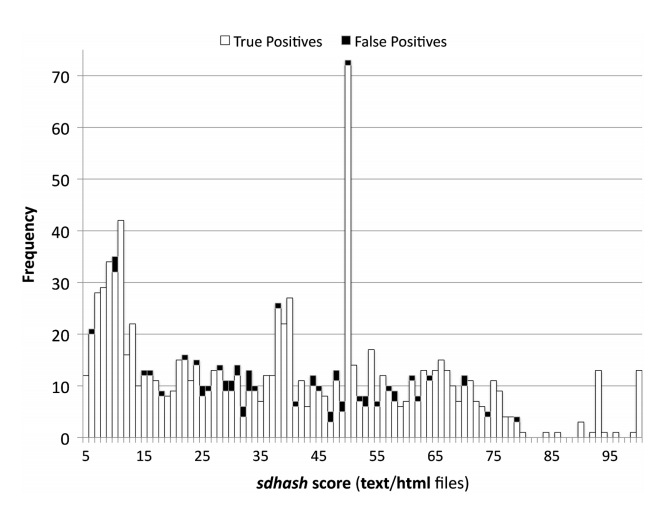
\includegraphics[scale=1]{Images/sdhash_TP_FP.jpg}}
\caption{Results of sdhash similarity score with HTML files.\label{fig:sdhash_tp_fp}}
\end{figure}

The only disadvantages of sdhash computation are the fact that the resulting hash size is directly proportional to the size of the file, which can be a problem when storing the hash (as we do), and the minimum file size requested for sdhash to work, which is 4096 B, a value that can't be satisfied when dealing with small configuration files uploaded (e.g., a .htaccess file).

\subsubsection{Ssdeep}
Ssdeep is one of the best-known techniques for detecting similar files. It's been invented by Jesse Kornblum \cite{ssdeep} in 2006 and based on the work on spam detection performed by Andrew Tridgell \cite{spamsum}.
The system is based on the concept of piecewise hashing. A piecewise hashing uses an arbitrary hashing algorithm (in ssdeep case is FNV) to create many checksums for a file instead than just one. Rather than generating a single hash for the entire file, a hash is generated for many discrete fixed-size segments of the file. Once we obtained all these pieces, ssdeep uses a rolling hash algorithm for creating a Context Triggered Piecewise Hash (CTPH). Such hashes can be compared in order to identify ordered homologous sequences between files.

This approach produces worse results than sdhash (ref~\ref{fig:sdhash_ssdeep}), but it has the advantage of obtaining a fixed-size hash (which is easier to store in a database) and it accepts files having a smaller size, 2048 B.

\begin{figure}[tbh]
\centerline{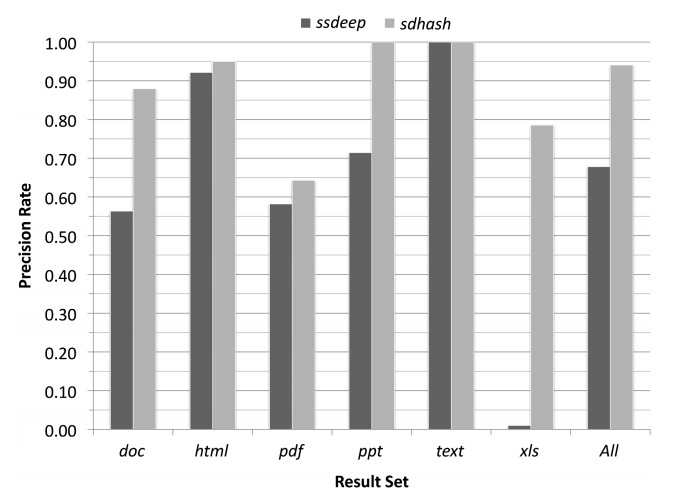
\includegraphics[scale=0.9]{Images/sdhash_ssdeep.jpg}}
\caption{Comparison of the precision rate of ssdeep and sdhash over different file types\label{fig:sdhash_ssdeep}}
\end{figure}

\subsubsection{MD5}
MD5 is a well-known technique for creating cryptographic hash of files. Designed by Ron Rivest and published by IETF as RFC 1321 \cite{md5}, this technique is based on different non-linear functions computed on fixed size input in order to achieve a 128 bit hash value.

This is the last technique we use for computing similarities: whenever the file is too short to apply sdhash or ssdeep, we use this algorithm in order to find if the normalized output of the file is the same of another file, showing its similarity.

\section{Visualization}

Our aim is to create a honeypot platform which can be easily deployed, updated and monitored by the administrator of the system. In order to accomplish the last action we created a web interface for monitoring the health of the system and obtain feedbacks from the analysis of data.

\subsection{Back-End Architecture}

We chose to use \emph{Node.Js} as platform for developing the webserver. \emph{Node.Js} is advertised on its website \cite{node_home} as
\begin{quotation}
Node.js is a platform built on Chrome's JavaScript runtime for easily building fast, scalable network applications. Node.js uses an event-driven, non-blocking I/O model that makes it lightweight and efficient, perfect for data-intensive real-time applications that run across distributed devices.
\end{quotation}

Its particular event-driven, non-blocking model, in fact, allows us to perform database queries and file analysis operations without involving waiting time from the end-user point of view. Furthermore, its modular nature and easiness of deployment makes the replication process fast and reliable.

We wanted to create a platform which does rely on a minimum number of external addition (other to the webserver) and which can perform several parallel queries to different databases for computing rankings and other operations. The system relies on \emph{Express} \cite{express_node} Framework, which is specifically aimed for minimality and flexibility, and uses only a few other modules, in the specific \emph{mysql} driver for Database communications and \emph{sanitizer}, a sanitizer library for strings.

Another requirement we imposed to our software is the possibility for it to work in a private network, disconnected from the Internet. For this reason, every library is provided directly by the webserver and there is no need to rely to any external server for the web interface to work.

\subsection{Front-End Architecture}

The Front-End architecture deeply relies on Javascript. We wanted to allow a good interactivity for the operator, who should be able to go from a high-level view to the single file analysis in a couple of clicks.

The interface uses Bootstrap \cite{bootstrap} framework: this is one of the most used front-end frameworks for web development, as it is able to create nice and clean web pages by creating a powerful templating system. It also manage interactions with end-users through several add-ons, like modals and accordions.

Graphs displaying is performed using D3 library \cite{d3_home} (acronym for Data-Driven Document), a library for displaying graphs as collections of SVG elements. Thanks to its emphasis on web standards, this library will work on all modern browsers (starting from Internet Explorer 8), without any issue, and avoiding to rely on proprietary frameworks for graph displaying. Other than static graphs like pie charts, this library is able to use heuristic algorithms in order  to show force-directed graphs, which have been one of our minimal requirements for clustering graphs visualization on our web interface.

\subsection{Overview}

Our dashboard should be able to give the following informations to the administrator: an overview over the current situation inside the system (files received, requests etc), an interactive graph showing in a clear way the various clusters, files the system failed to clusterize, stats about the system (requests, common referrers, attackers provenance..). In the following we will give three examples of the functionalities of the interface.

\begin{figure}[tbh]
\centerline{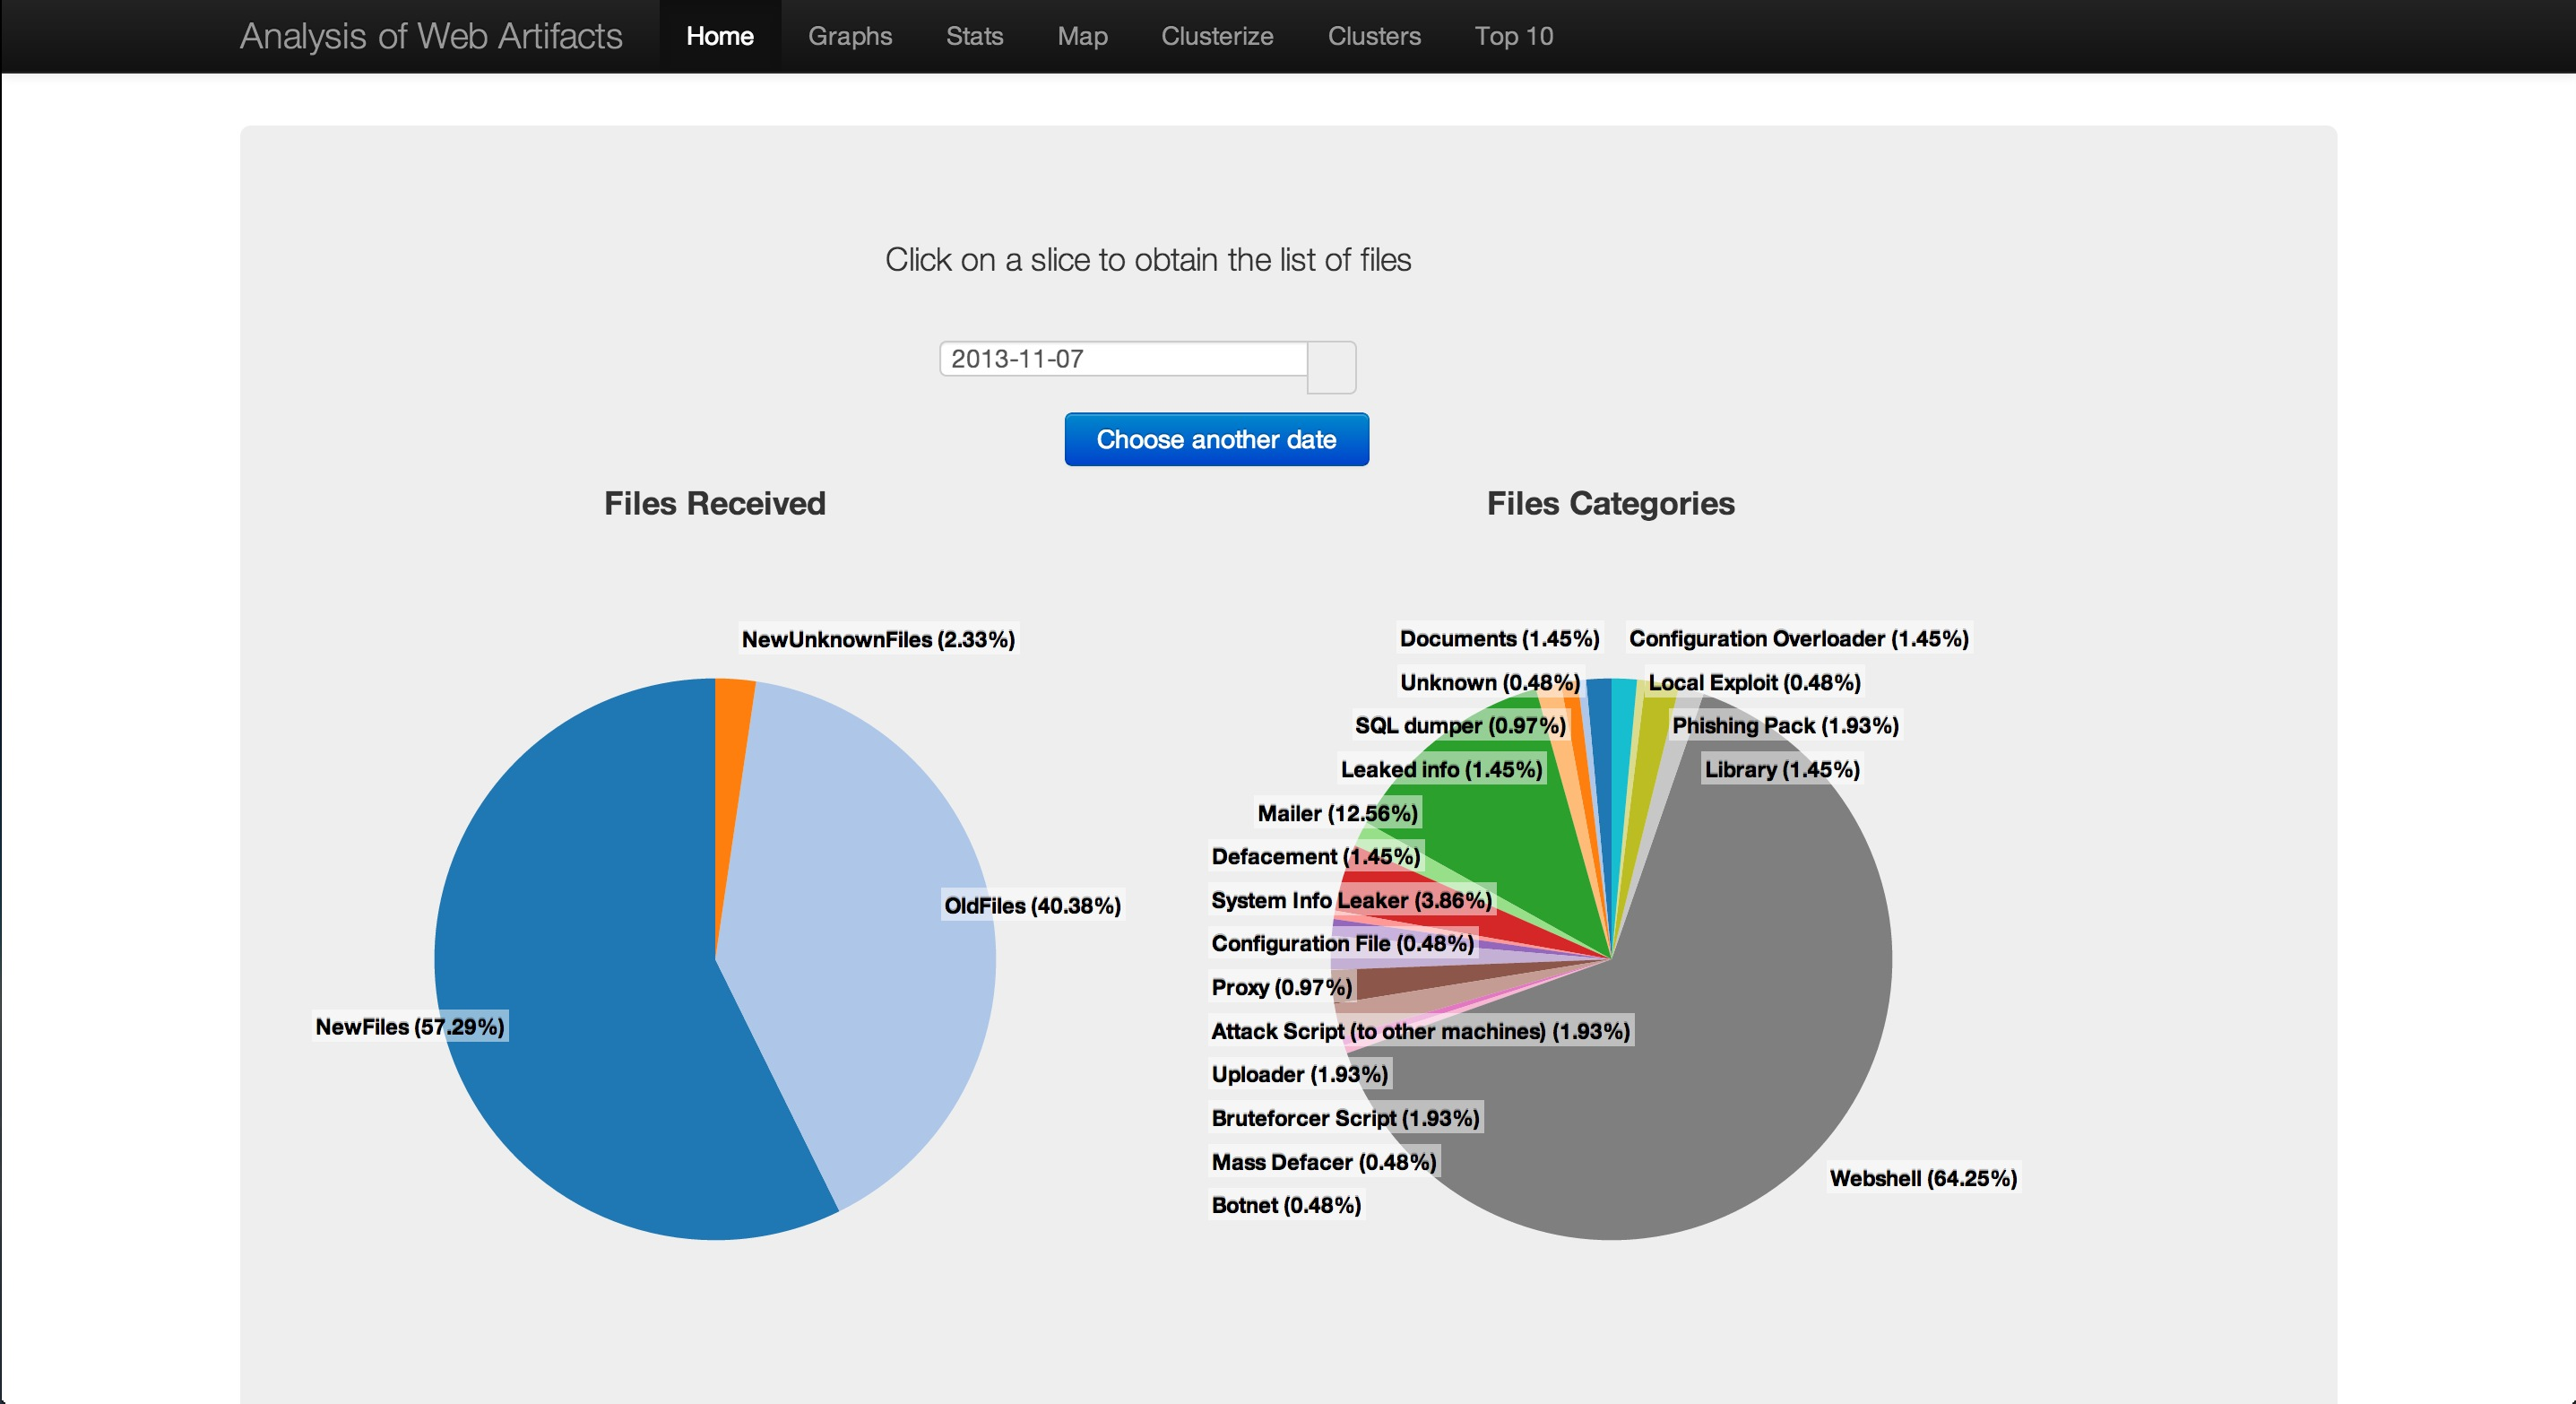
\includegraphics[scale=0.2]{Images/honeyFace_home.jpg}}
\caption{Screenshot of the web interface home page\label{fig:web_home}}
\end{figure}

The homepage(ref~\ref{fig:web_home}) of the web interface displays several pie charts, the most important being the number of file received during the day, divided among three categories, oldFiles (files that were already present in our databases), newFiles (new files received for which our clusterization system already categorized) and newUnknownFiles (new files that our system was unable to clusterize), and the result of our categorization for the files received during the day. Clicking on a slice of a pie displays a list of files belonging to that tranche, with the possibility to display details for each file.

\begin{figure}[tbh]
\centerline{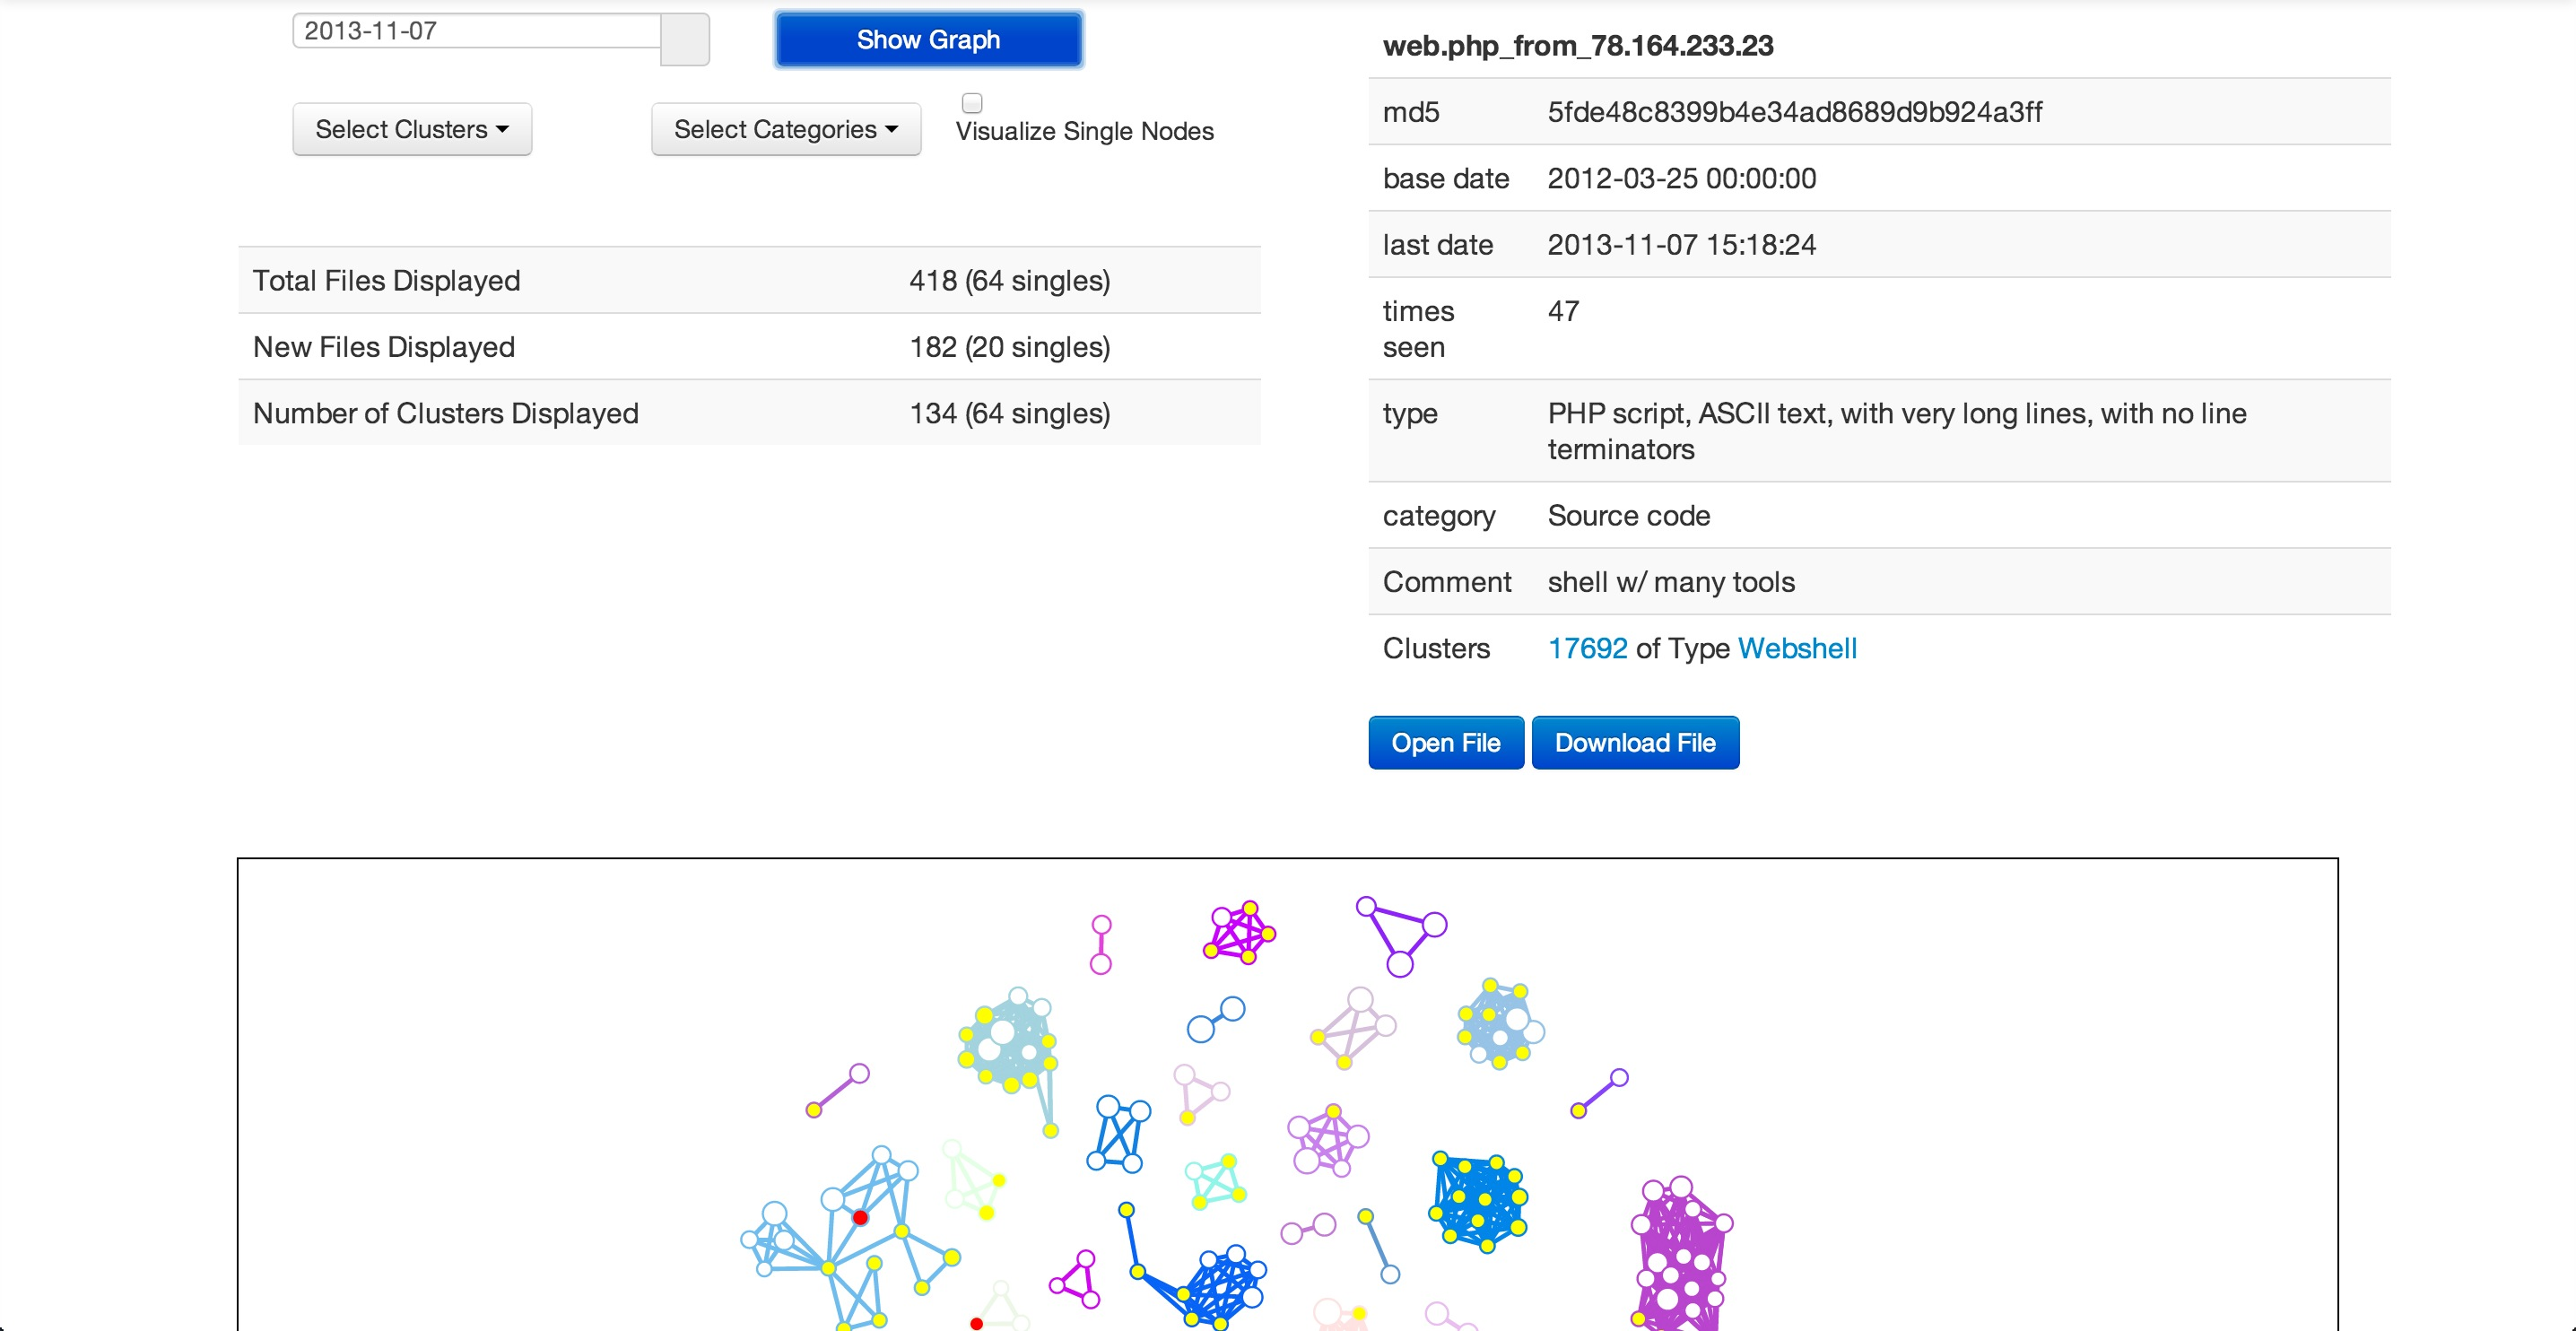
\includegraphics[scale=0.2]{Images/honeyFace_graph.jpg}}
\caption{Screenshot of a graph created by the web interface\label{fig:web_graph}}
\end{figure}

The Graph page (ref~\ref{fig:web_graph}) displays a force-directed graph showing the different clusters. It is possible to choose several parameters for the display, like the categories to be displayed and the file types. We chose to display files received only in the last 15 days with respect to the date chosen, in order not to overload the browser (the map is interactive and it's built client-side).

We can display details about a single file through the single file web page. We can see several details about the file, type, clusters, date received etc. We also have the possibility to write a comment about the file.
One of The most interesting features we provide on this page is the possibility to use ``Transformer'' over the single file (ref~\ref{fig:deobfDouble}), obtaining a rapid feedback over how our system managed the single file and in order to get a better understanding over the code.

\begin{figure}
\centering
\begin{subfigure}{.5\textwidth}
  \centering
  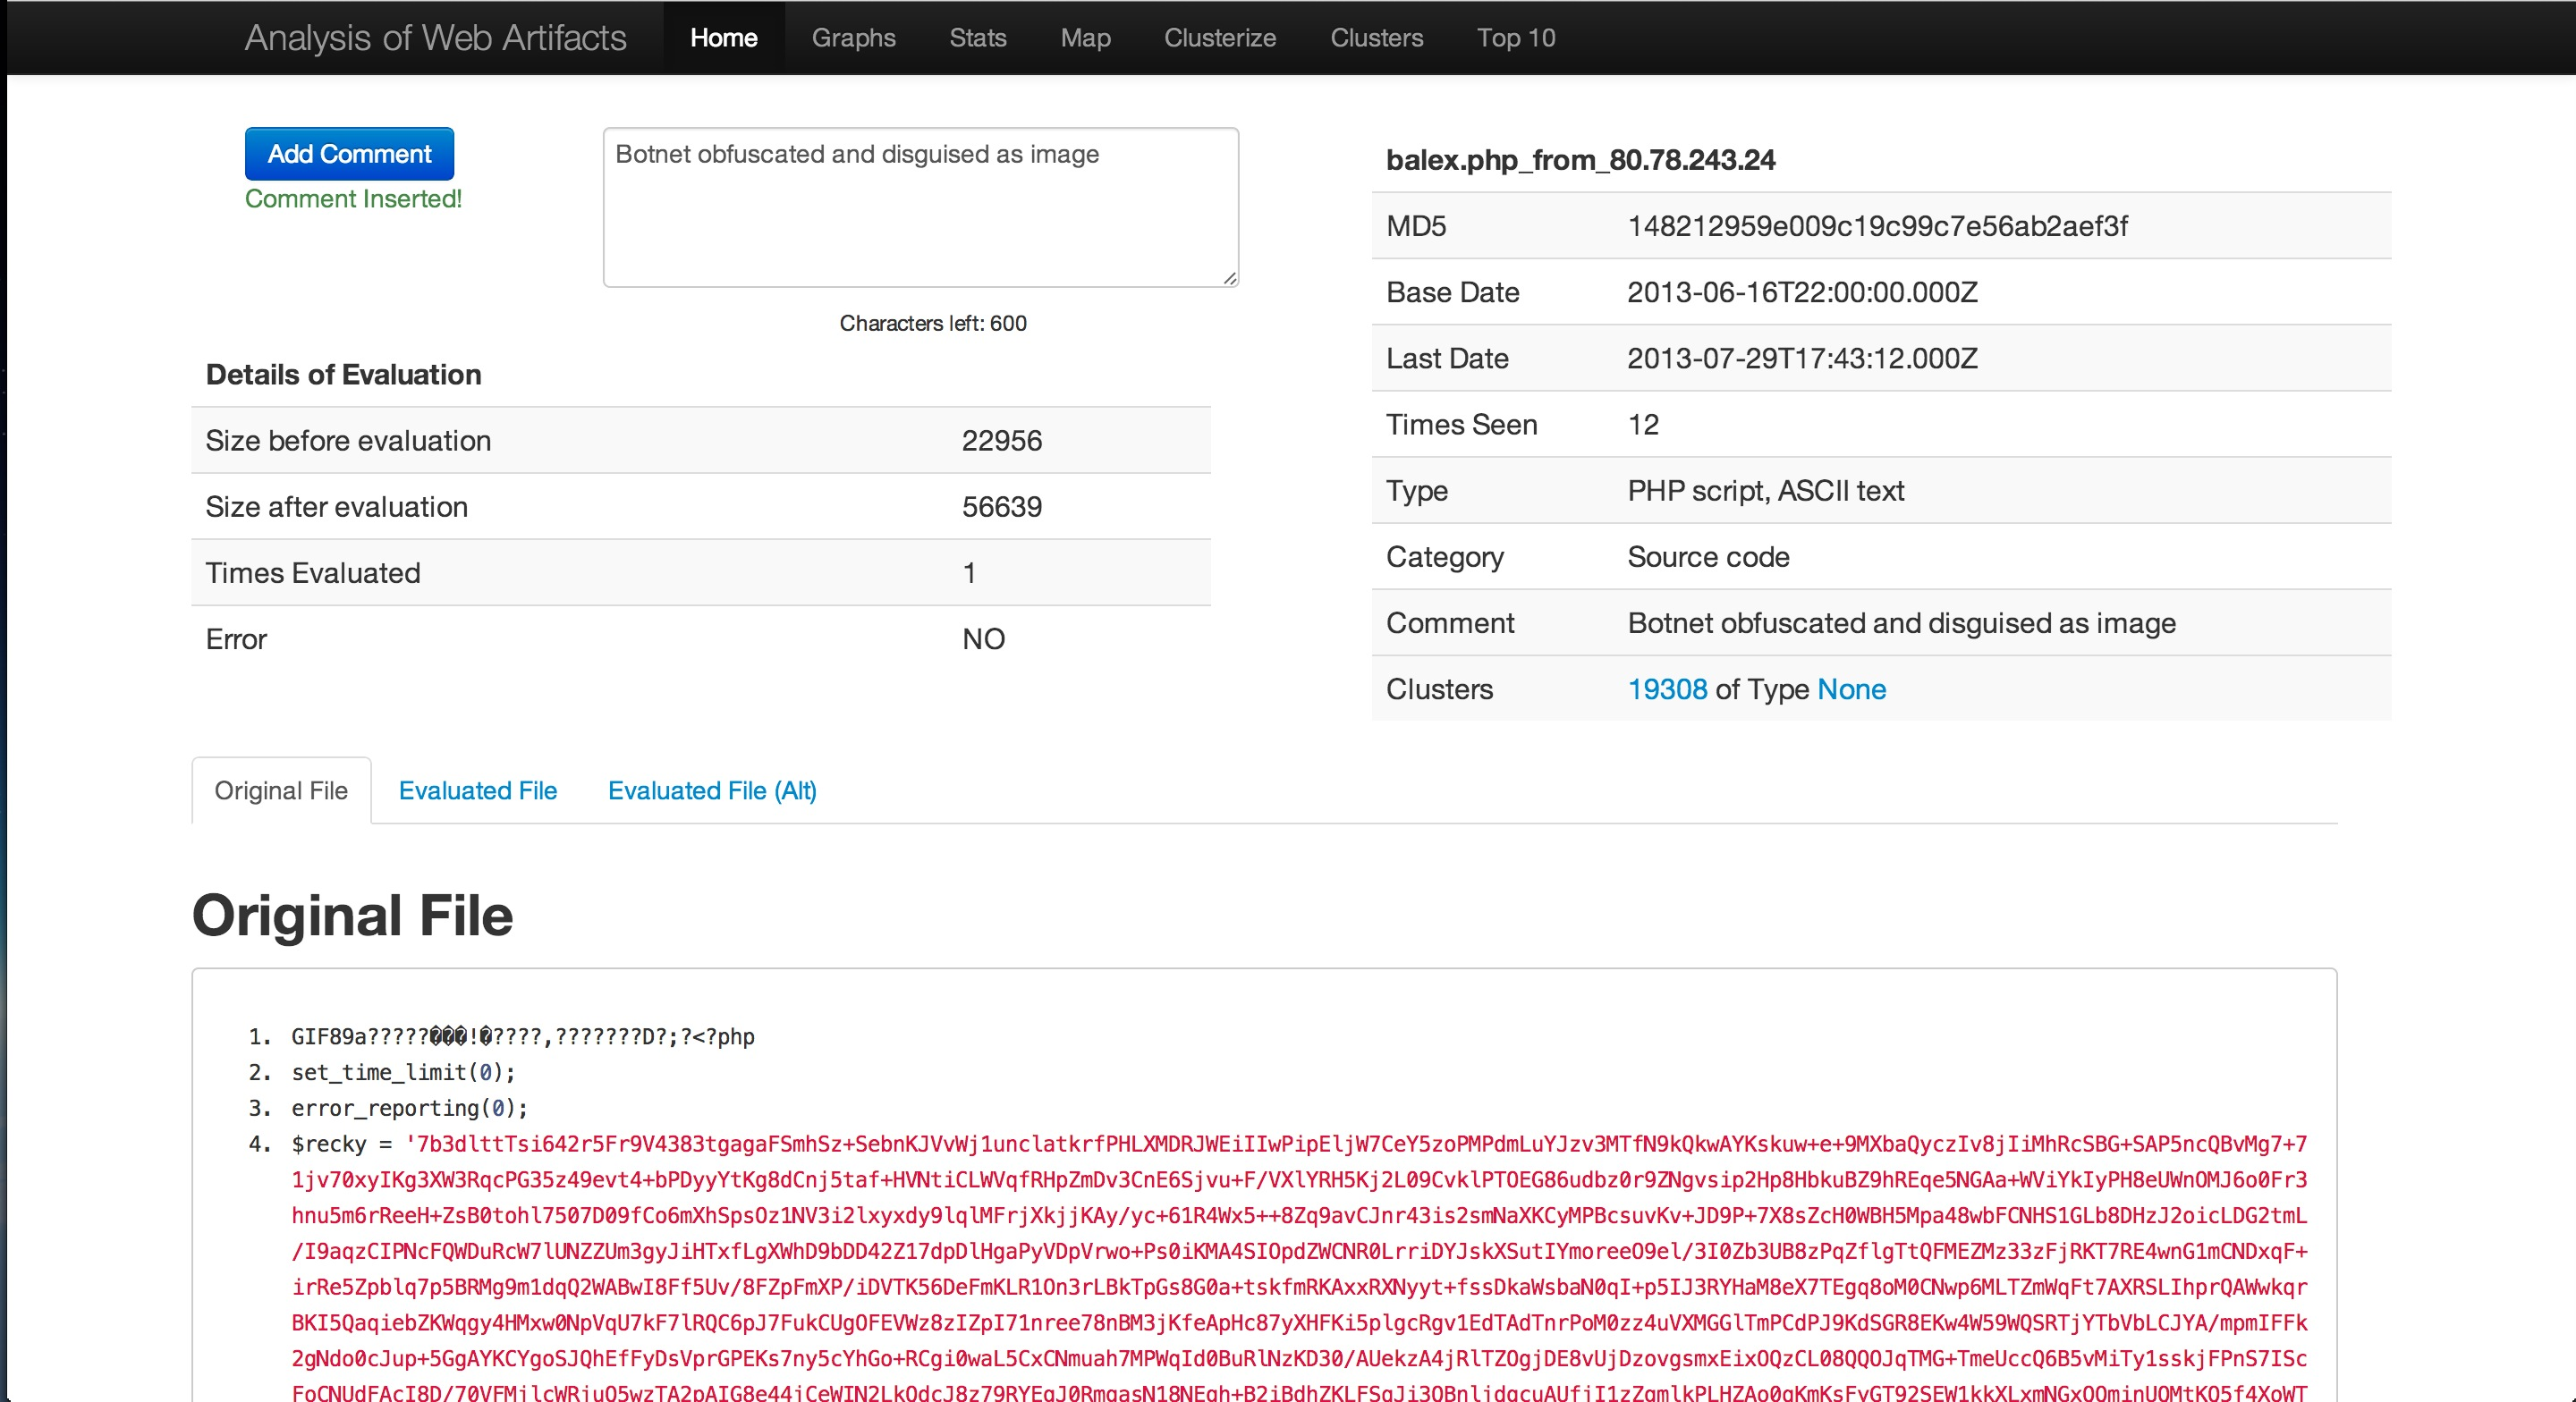
\includegraphics[width=1.0\linewidth]{Images/obf_file.jpg}
  \caption{Before deobfuscation}
  \label{fig:sub1}
\end{subfigure}%
\begin{subfigure}{.5\textwidth}
  \centering
  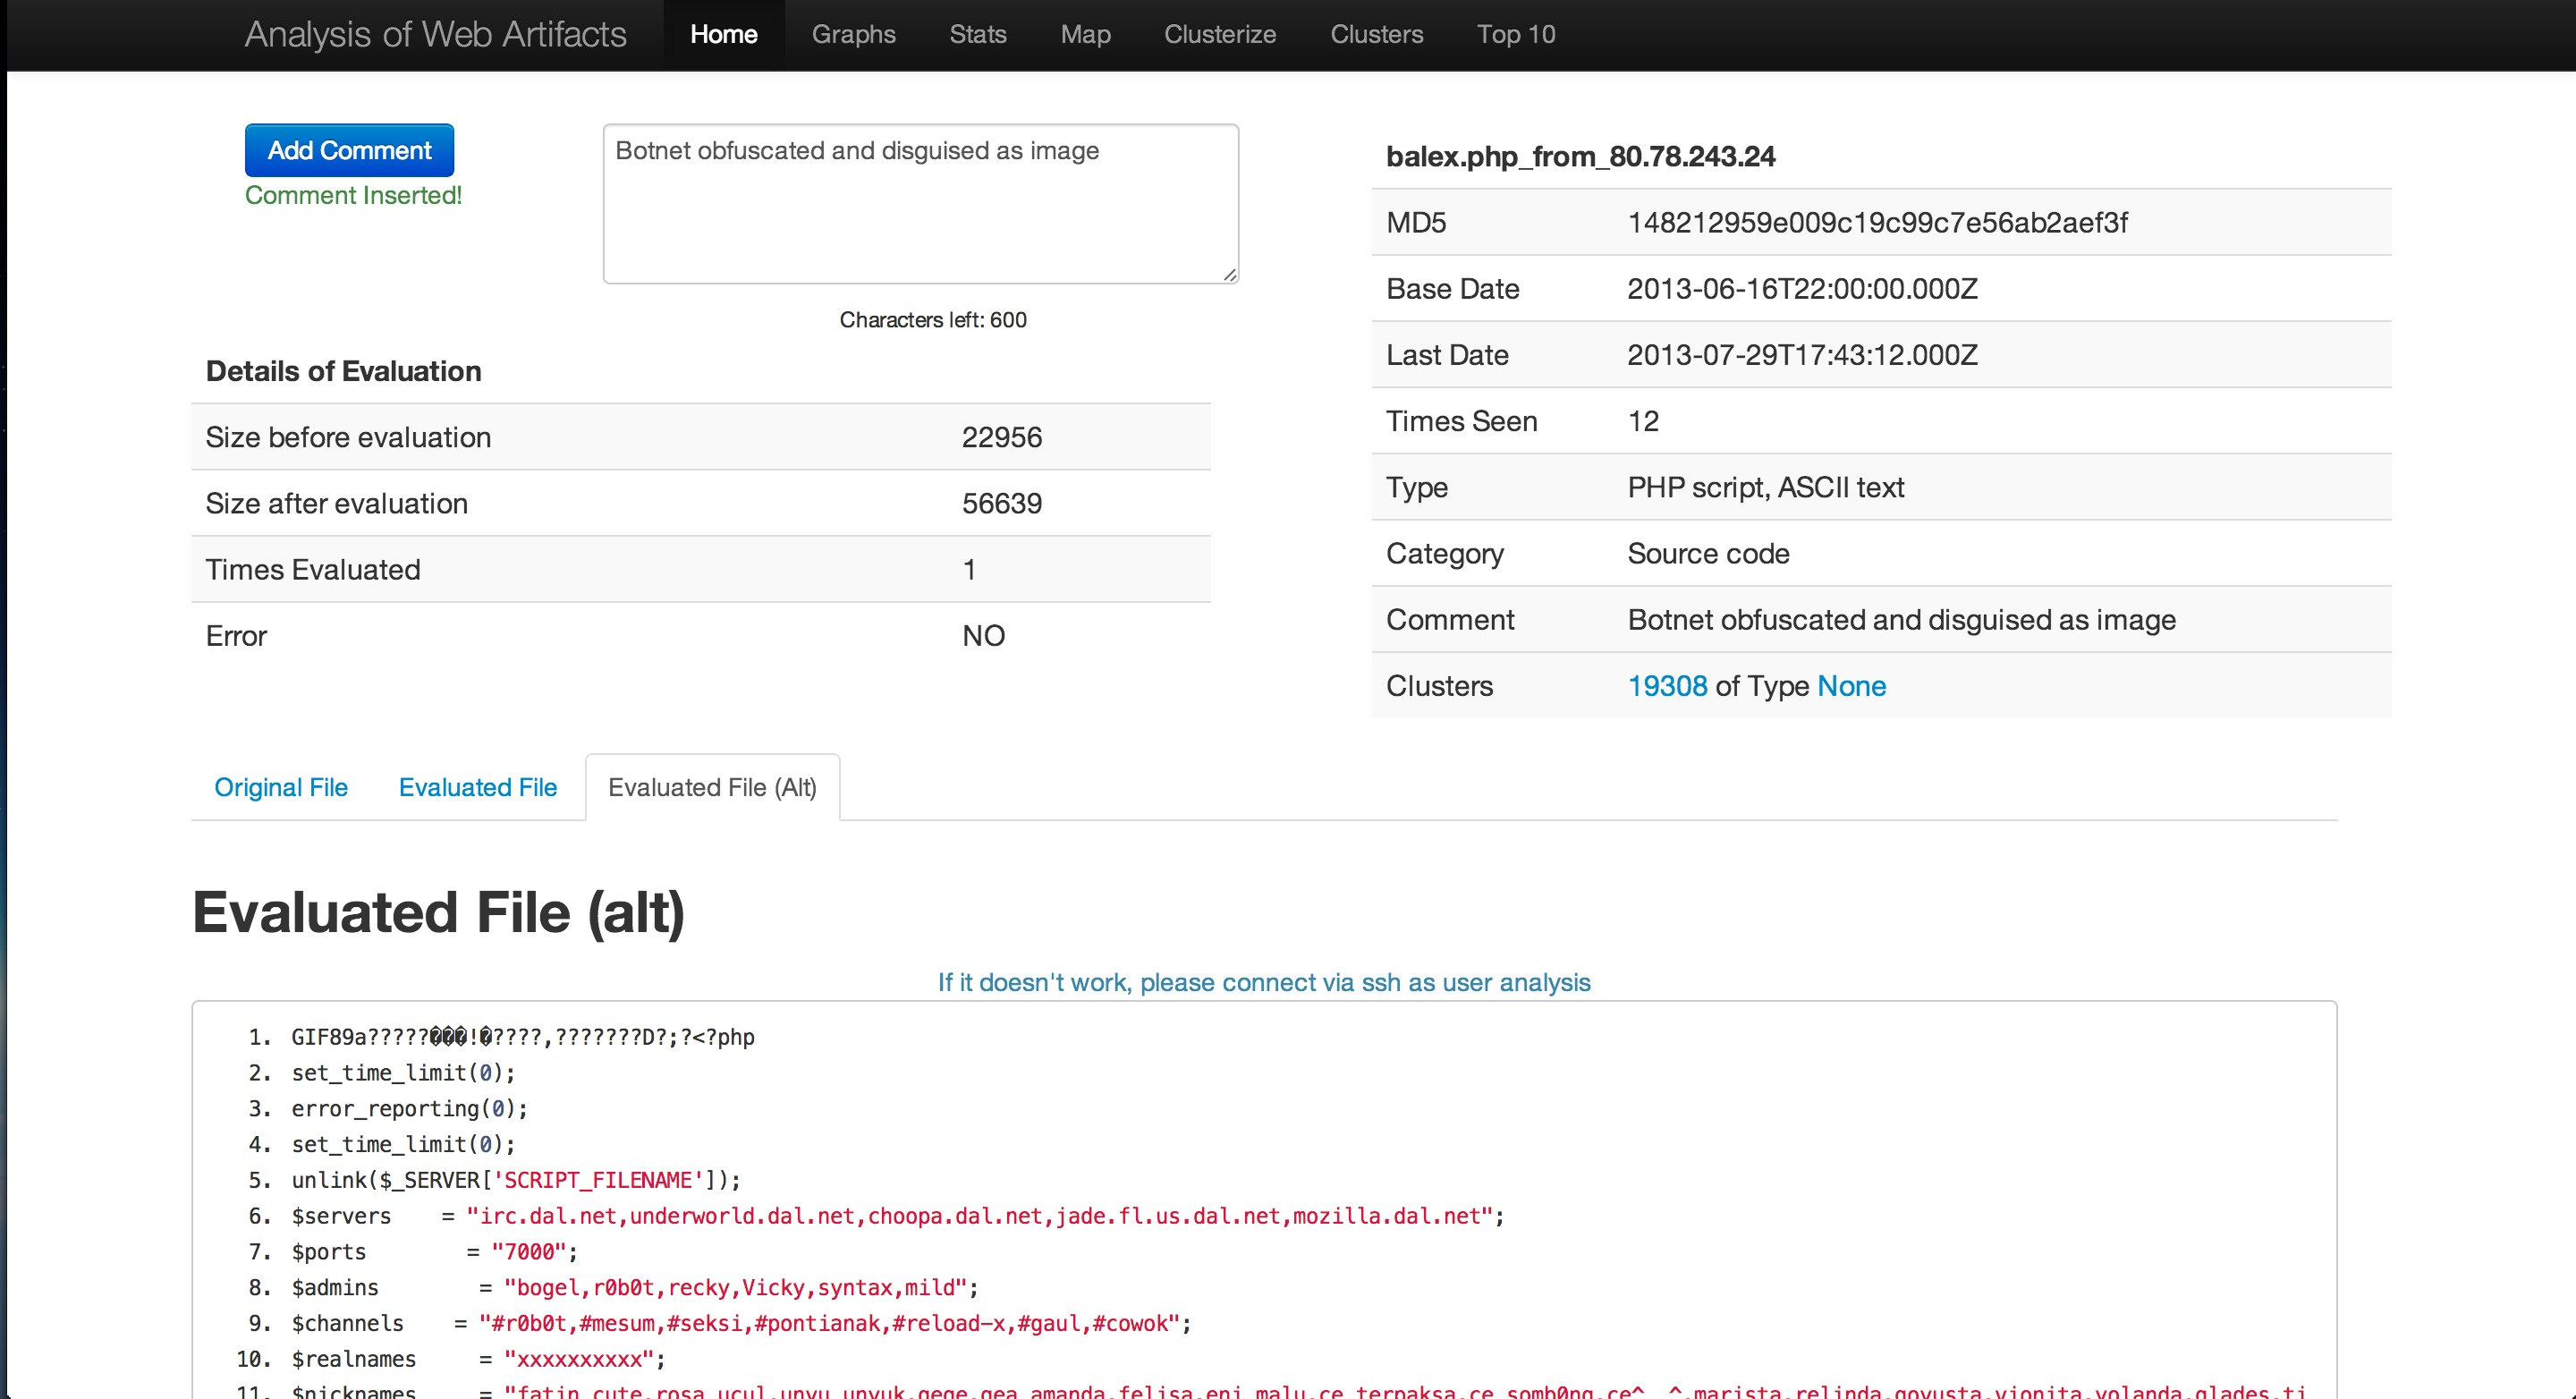
\includegraphics[width=1.0\linewidth]{Images/deobf_file.jpg}
  \caption{After deobfuscation}
  \label{fig:sub2}
\end{subfigure}
\caption{Example of the Single File web page}
\label{fig:deobfDouble}
\end{figure}
